\documentclass[UTF8,zihao=-4,a4paper,fontset=fandol]{ctexart}
\usepackage{cumcm-paper}
\emergencystretch=2em
\title{系泊系统的静力响应与鲁棒优化设计}
\author{}
\date{}

\begin{document}
\maketitle

\begin{cumcmabstract}
近浅海传输节点的工作性能同时受浮标吃水、刚性构件姿态、锚链形态和环境载荷影响。本文建立浮标--钢管--钢桶--重物球--锚链的一体化静力模型：以构件水中有效重量修正重力，以刚体力矩平衡递推钢桶和钢管倾角，以分段悬链线刻画锚链铺底与全悬状态，并在复杂环境下进一步引入风流空间向量、姿态相关迎流面积和多工况鲁棒优化。

针对问题一，在水深18 m、II型锚链22.05 m和1200 kg重物球条件下，求解浮标吃水、五个刚性构件倾角及锚链形状。风速12 m/s时钢桶倾角为$1.0073^\circ$、吃水为0.7348 m、游动半径为14.3029 m，锚链铺底6.8246 m；风速24 m/s时相应结果为$3.8461^\circ$、0.7489 m和17.4232 m，铺底长度仅0.3233 m。210链环离散模型与连续悬链线结果的关键指标相对误差均很小，验证了连续模型的适用性。

针对问题二，在36 m/s风速下原1200 kg方案的钢桶倾角和锚点夹角分别达到$8.0636^\circ$和$17.9006^\circ$，均超过限制。将重物球质量作为决策变量，建立带静力平衡和水深闭合约束的最小配重模型。锚点角约束对应临界质量1524.0332 kg，钢桶角约束对应1780.8803 kg，故可行质量下界和理论最优值均为1780.8803 kg；考虑配重取整，推荐1800 kg，此时两角分别为$4.9276^\circ$和$14.1945^\circ$。

针对问题三，考虑16--20 m水深、最大36 m/s风速和1.5 m/s流速，建立三维风流载荷与构件姿态耦合模型，并枚举整数链环、配重档位与环境组合。经204个可行设计的Pareto筛选和180个代表工况复核，推荐IV型锚链22.05 m、重物球4050 kg。该方案的最大钢桶倾角为$4.7382^\circ$，最大锚点夹角为$14.8547^\circ$，最大吃水为1.7519 m，最大游动半径为19.6195 m；浅水控制游动范围和钢桶倾角，深水控制吃水和锚点夹角。
\aimark{1}
\end{cumcmabstract}

\keywords{系泊系统；悬链线；静力平衡；鲁棒优化；Pareto前沿}
\CumcmBodyStart

\section{问题重述}
近浅海观测网传输节点由圆柱形浮标、四节钢管、密封钢桶、重物球、锚链及锚组成。浮标承担水面风载并提供浮力，水声设备安装于钢桶内；钢桶倾角超过$5^\circ$时工作效果变差，锚链在锚点处与海床夹角超过$16^\circ$时锚可能被拖行。设计任务是在给定海洋环境中确定链型、链长和配重，使系统满足安全约束，并减小浮标吃水、游动范围和钢桶倾角。

问题一要求验证给定的II型锚链22.05 m和1200 kg配重在12 m/s、24 m/s风速下的静态响应。问题二将风速提高至36 m/s，需要判断原方案并寻找满足两个角度限制的配重质量。问题三进一步考虑16--20 m水深、最大1.5 m/s水流及不同风流方向，完成链型、链长和配重的综合设计，并分析不同工况下的构件姿态、锚链形态、吃水和游动区域。

\section{总体分析与统一建模路线}
三问共享同一物理链条：环境水平载荷决定浮标底部连接力，连接力与构件水中重量共同决定钢管和钢桶姿态，刚性构件端点位置又与锚链悬链线及水深约束闭合。问题一在静水条件下建立二维基准模型；问题二保持结构不变，仅把配重提升为优化变量；问题三在基准模型上增加水流分布载荷、水平向量递推、链型离散选择和多工况搜索。

计算中先给定锚链顶端或锚点竖直张力，由下向上递推竖直载荷并计算浮标吃水，再由吃水更新迎风面积；随后求各刚性构件角度与空间投影，最后使用水深闭合方程求未知张力或悬起链长。锚链优先按部分铺底状态求解，若所需悬起长度超过总链长，则自动切换至完全悬链。该状态切换贯穿三问，避免把不同载荷状态强行套用同一边界条件。
\aimark{2}

\section{模型假设}
\begin{enumerate}
\item 系统在稳定风流作用下达到静态平衡，忽略波浪、瞬态振动和构件惯性；
\item 浮标依靠自身浮稳性保持竖直，只考虑吃水变化和水平移动；
\item 钢管和钢桶为刚性圆柱构件，连接处为理想铰，重物球作为钢桶下端集中载荷；
\item 锚链均匀、不可伸长且只承受拉力，海床水平并忽略链床摩擦；
\item 钢管和钢桶按外部圆柱体积计算浮力；题目未给出重物球和锚链排水体积，主模型忽略二者浮力；
\item 问题三水流速度沿水深均匀，钢管和钢桶水流合力作用于几何中心；因缺少尺寸，忽略重物球和锚链自身水流力。
\end{enumerate}

\section{主要符号}
\begin{table}[H]\centering
\caption{主要符号及含义}
\label{tab:symbols}
\begin{tabular}{ccc}
\toprule
符号 & 含义 & 单位\\
\midrule
$h$ & 浮标吃水深度 & m\\
$H,V$ & 张力的水平、竖直分量 & N\\
$\theta_i,\theta_b$ & 第$i$节钢管、钢桶相对竖直方向的倾角 & $^\circ$\\
$L_c,q$ & 锚链总长、单位长度有效重量 & m，N/m\\
$V_a,V_t$ & 锚点、锚链顶端竖直张力 & N\\
$R$ & 浮标相对锚点的水平偏移模长 & m\\
$d,v_w,v_c,\varphi$ & 水深、风速、流速、风流夹角 & m，m/s，m/s，$^\circ$\\
\bottomrule
\end{tabular}
\end{table}

\section{问题一：静水风载下的系统响应}
\subsection{本问分析}
问题一给定II型锚链22.05 m、重物球1200 kg、水深18 m和静水条件，要求在12 m/s与24 m/s风速下计算浮标吃水、各刚性构件倾角、锚链形状和游动区域。其耦合关系为：吃水决定露出水面的迎风面积，风力决定水平张力；下部构件和悬起锚链的竖直载荷决定浮标吃水；构件姿态与锚链高度共同满足18 m水深闭合。

\subsection{浮标与刚性构件平衡}
设浮标吃水为 \(h\)，其浮力和风荷载分别为

\[
B_f=\rho g\pi h,
\qquad
H=1.25(2-h)v^2. \tag{1}
\]
钢管、钢桶按封闭圆柱的外形体积计算浮力，每节钢管和钢桶的水中有效重量分别为

\[
W_p=78.3566\ \mathrm N,
\qquad W_b=270.2363\ \mathrm N.
\]
题目没有提供重物球体积，故将其作为钢桶下端的独立集中载荷并忽略浮力，取

\[
W_s=1200g=11772\ \mathrm N.
\]
对于任一刚性构件，设上下端竖直张力为 \(V_u,V_l\)，则

\[
V_u=V_l+W,
\qquad
\tan\theta=\frac{2H}{V_u+V_l}. \tag{2}
\]
锚链顶端竖直张力为 \(V_t\) 时，钢桶下端载荷为

\[
V_{b,l}=V_t+W_s.
\]
由钢桶向上逐节递推四节钢管，得到下部系统对浮标的竖直拉力

\[
V_0=V_t+W_s+W_b+4W_p. \tag{3}
\]
浮标竖直平衡给出

\[
h=\frac{1000g+V_0}{\rho g\pi}. \tag{4}
\]
式（1）和式（4）形成吃水与水平风载之间的反馈。

\subsection{锚链形状与状态判断}
II型锚链单位长度质量为7 kg/m，忽略锚链浮力后

\[
q=7g=68.67\ \mathrm{N/m}.
\]
若存在铺底段，设悬起链长为 \(l\)，离床点处切线水平，则

\[
V_t=ql,
\]
\[
x_c=\frac{H}{q}\operatorname{arsinh}\frac{ql}{H},
\]
\[
y_c=\frac{H}{q}
\left[
\sqrt{1+\left(\frac{ql}{H}\right)^2}-1
\right]. \tag{5}
\]
水深闭合条件为

\[
h+y_c+\cos\theta_b+
\sum_{i=1}^{4}\cos\theta_i=18. \tag{6}
\]
由式（6）求出 \(l\)。若 \(l\le22.05\)，铺底假设成立；若超过总链长，则转入全悬链模型。本问两种风速求得的悬起链长均小于总长，因此锚点处切线水平，锚点角为零。

浮标游动半径由铺底链段、悬起链段及五个刚性构件的水平投影组成：

\[
R=(22.05-l)+x_c+\sin\theta_b+
\sum_{i=1}^{4}\sin\theta_i. \tag{7}
\]
游动圆面积取 \(A=\pi R^2\)。

\subsection{求解结果}
\begin{table}[H]\centering\small
\caption{问题一两种风速下的系统平衡状态}
\label{tab:q1-1}
\begin{tabular}{ccc}
\toprule
指标 & 12 m/s & 24 m/s \\
\midrule
吃水深度/m & 0.7348 & 0.7489 \\
第1节钢管倾角/(°) & 0.9764 & 3.7324 \\
第2节钢管倾角/(°) & 0.9822 & 3.7536 \\
第3节钢管倾角/(°) & 0.9880 & 3.7751 \\
第4节钢管倾角/(°) & 0.9939 & 3.7968 \\
钢桶倾角/(°) & 1.0073 & 3.8461 \\
悬起链长/m & 15.2254 & 21.7267 \\
铺底链长/m & 6.8246 & 0.3233 \\
游动半径/m & 14.3029 & 17.4232 \\
游动圆面积/m² & 642.68 & 953.68 \\
\bottomrule
\end{tabular}
\end{table}
风速加倍后，风荷载近似增至4倍，构件倾角和游动半径明显增大，铺底长度由6.8246 m减小至0.3233 m；浮标吃水仅增加0.0141 m，说明风速主要改变水平载荷。24 m/s工况已接近锚链完全离床临界状态，但铺底长度仍为正，采用部分铺底模型自洽。

两种工况的链形可由式（5）直接参数化。12 m/s时$H/q=3.3164$ m，铺底段终点位于$x=6.8246$ m，悬链段延伸至$x=14.2165$ m并升高12.2660 m；24 m/s时$H/q=13.1176$ m，铺底段终点移至$x=0.3233$ m，悬链段延伸至$x=17.0935$ m并升高12.2620 m。风速增加使特征长度$H/q$明显增大，链形趋于平缓并向水平方向展开，而顶端高度因18 m水深闭合保持接近。该参数变化与图\ref{fig:q1-chain}所示曲线一致，也解释了游动半径增加而吃水变化较小的原因。

\subsection{连续模型验证}
II型锚链单环长度为0.105 m，总长对应210个链环。将锚链离散为短柔性单元，以单元两端竖直张力平均值确定其方向，并与浮标、刚性构件和水深方程联立。连续与离散模型在12 m/s、24 m/s下的游动半径相对误差分别为0.000818\%和0.000145\%，钢桶与钢管倾角相对误差均小于0.0001\%。最大相对误差出现在24 m/s的铺底长度，为0.010738\%，但绝对差仅 \(3.47\times10^{-5}\) m。由此说明连续悬链线足以用于后续配重搜索和多工况设计。

校核数据共比较两种风速下的吃水、水平张力、悬起链长、铺底链长、锚链跨度与高度、五个构件倾角及游动半径等24项指标。12 m/s工况的最大相对误差为0.002043\%，对应铺底长度；24 m/s工况的最大相对误差为0.010738\%，同样对应铺底长度。铺底长度是总链长与悬起链长之差，在24 m/s时仅为0.3233 m，较小的绝对误差除以接近零的铺底长度会放大相对误差，因此不能据此判断连续模型失效。更直接影响结论的游动半径、吃水和钢桶倾角均保持更高一致性，且两种模型对“仍有铺底链段”的状态判定相同。

连续模型与离散模型的误差方向也具有可解释性。链环模型用有限个线段逼近光滑悬链线，节点处方向离散会使水平跨度和离床位置产生微小偏差；随着链环数量增加，这类几何误差应收敛。由于本题已由实际210个链环完成离散，比较并非任意网格试算，而是对应题设结构的独立复算。校核的目的在于确认连续悬链线不会改变主要响应和状态边界，不把远低于测量尺度的数值差异包装成工程精度。

\subsection{求解流程、结果解释与适用范围}
给定悬起链长后，程序由锚链顶端向上递推钢桶、四节钢管及浮标的竖直张力和倾角，并同步更新吃水与风荷载；外层用二分法使总竖直高度等于18 m。若悬起长度超出总链长，才切换到完全悬起模型。本问两种风速均落在部分铺底分支，并通过受力、力矩和水深闭合检查。

风速由12 m/s增至24 m/s后，悬起链长增加6.5013 m，而吃水仅增加0.0141 m，说明游动范围和铺底长度比吃水更敏感。24 m/s时仅余0.3233 m锚链铺底，提示更高风速下必须允许状态切换。210链环离散复算与连续模型的关键响应相对误差均小于0.011\%，支持后续批量计算采用连续悬链线。

模型只描述稳定风作用下的静态平衡，不能刻画结构惯性、阵风峰值和链环接触滞回；理想柔索近似也忽略轴向伸长与弯曲刚度。离散校核仅证明连续悬链线在当前稳态工况下的一致性，不代表动态响应和疲劳安全性。

\subsection{本问结论}
在静水和给定结构条件下，12 m/s与24 m/s风速对应的钢桶倾角分别为 \(1.0073^\circ\) 与 \(3.8461^\circ\)，浮标吃水分别为0.7348 m与0.7489 m，游动半径分别为14.3029 m与17.4232 m。两种工况锚链均有铺底段，锚点夹角为零；24 m/s工况更接近整链悬起，是进入问题二极端风速分析的基础。
\aimark{3}

\begin{figure}[H]\centering
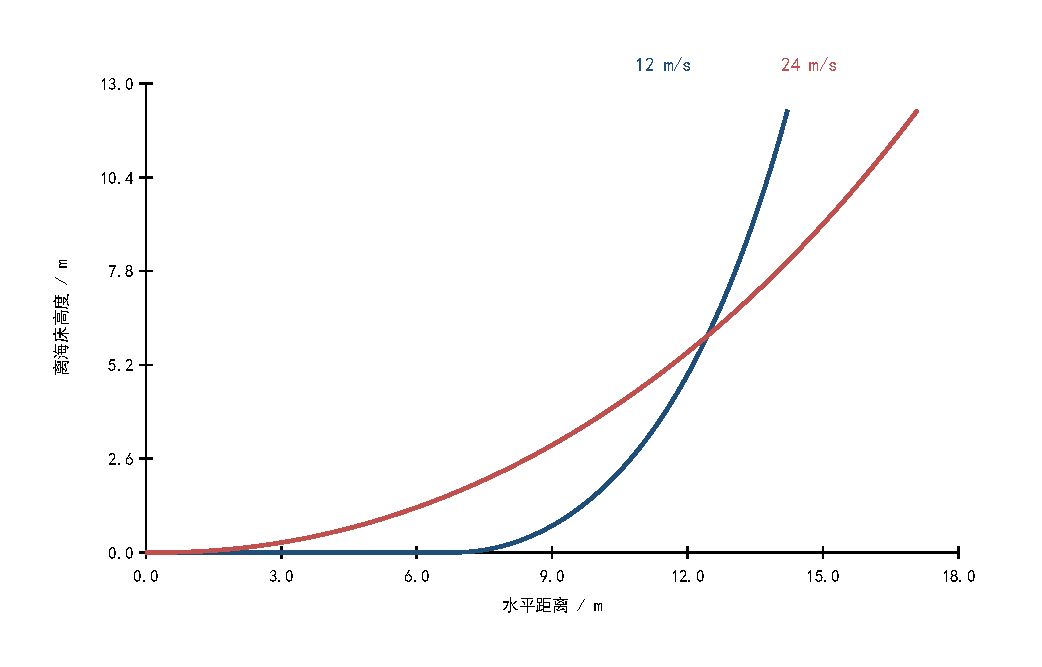
\includegraphics[width=0.78\textwidth]{../figures/question-1-chain-profiles.pdf}
\caption{问题一两种风速下的锚链形状}
\label{fig:q1-chain}
\end{figure}

\section{问题二：极端风速下的最小配重}
\subsection{问题分析}
问题二沿用问题一的结构参数和环境假设，将海面风速提高到 36 m/s。由于问题一明确规定海水静止，本问水流速度为零，故水流力为零。需要先计算原 1200 kg 重物球方案下钢桶、四节钢管、锚链和浮标的平衡状态，再调节重物球质量，使钢桶倾角不超过 \(5^\circ\)，且锚链在锚点处与海床的夹角不超过 \(16^\circ\)。

增加配重能够增大钢桶两端的竖直张力，使钢桶更接近竖直；同时，配重增加会使浮标吃水加深，浮标露出水面的迎风面积减小，从而降低水平风荷载。因此，重物球质量通过竖直载荷和风荷载两条途径共同影响系统姿态。本问将重物球质量作为设计变量，在满足两个角度约束的质量范围内寻找最小质量。

\subsection{模型假设}
本问沿用问题一的基本假设：系统处于二维静态平衡；浮标依靠自身浮稳性保持竖直；钢管和钢桶为铰接刚性构件；重物球是钢桶下端连接点处的独立集中载荷；锚链为均匀、不可伸长的柔索；忽略波浪、海床摩擦、锚链浮力和重物球浮力。

此外，由于海水静止，题目给出的水流力公式在本问中取

\[
F_c=374S_cv_c^2=0.
\]
系统水平环境载荷仅来自浮标露出水面部分受到的风力。

\subsection{36 m/s风荷载模型}
设浮标吃水深度为 \(h\)。浮标直径为2 m、高2 m，保持竖直时露出水面的高度为 \(2-h\)，迎风投影面积为

\[
S_w=2(2-h).
\]
根据题目给出的近海风荷载公式，36 m/s风速下的风力为

\[
F_w=0.625S_wv^2
=0.625\times2(2-h)\times36^2,
\]
即

\[
H=F_w=1620(2-h). \tag{1}
\]
式（1）中的 \(H\) 也是系泊系统张力的水平分量。由于配重质量影响吃水深度，风力不能预先设置为固定常数，而应在每次平衡计算中根据 \(h\) 更新。

\subsection{原1200 kg方案的平衡状态}
将 \(m_s=1200\ \mathrm{kg}\) 代入问题一模型。计算表明，36 m/s时整条22.05 m锚链已经离开海床，因此必须使用完全悬链模型，而不能继续采用锚点切线水平的部分铺底模型。

原方案的浮标吃水为0.7700 m，水平风荷载为1992.62 N，浮标游动半径为18.7145 m；钢桶倾角和锚点夹角分别为$8.0636^\circ$和$17.9006^\circ$。
原方案的钢桶倾角满足

\[
8.0636^\circ>5^\circ,
\]
锚点夹角满足

\[
17.9006^\circ>16^\circ.
\]
因此原1200 kg重物球同时违反两个约束，需要增加配重质量。

\subsection{完全悬链模型}
设锚点处张力的水平和竖直分量分别为 \(H\) 和 \(V_a\)，锚链单位长度有效重量为

\[
q=7g=68.67\ \mathrm{N/m},
\]
总长度为 \(L_c=22.05\ \mathrm m\)。锚链顶端竖直张力为

\[
V_t=V_a+qL_c. \tag{2}
\]
完全悬链的水平跨度为

\[
x_c=\frac{H}{q}
\left[
\operatorname{arsinh}\left(\frac{V_t}{H}\right)
-\operatorname{arsinh}\left(\frac{V_a}{H}\right)
\right], \tag{3}
\]
竖直高度为

\[
y_c=\frac{1}{q}
\left[
\sqrt{H^2+V_t^2}-\sqrt{H^2+V_a^2}
\right]. \tag{4}
\]
锚点处锚链切线与海床的夹角为

\[
\alpha_a=\arctan\frac{V_a}{H}. \tag{5}
\]
以锚点为坐标原点，锚链形状为

\[
y(x)=a\left[
\cosh\left(\frac{x}{a}+b\right)-\cosh b
\right], \tag{6}
\]
其中

\[
a=\frac{H}{q},
\qquad
b=\operatorname{arsinh}\frac{V_a}{H}.
\]
\subsection{重物球质量与刚性构件平衡}
将重物球质量记为 \(m_s\)，忽略重物球浮力，则重物球在钢桶下端施加的集中载荷为

\[
W_s=m_sg. \tag{7}
\]
钢桶下端竖直载荷为

\[
V_{b,l}=V_t+m_sg. \tag{8}
\]
钢桶水中有效重量为 \(W_b=270.2363\ \mathrm N\)，故其上端竖直张力为

\[
V_{b,u}=V_{b,l}+W_b. \tag{9}
\]
由钢桶质心力矩平衡，其倾角满足

\[
\theta_b=\arctan
\frac{2H}{V_{b,l}+V_{b,u}}. \tag{10}
\]
四节钢管从第4节向第1节逐节递推。每节钢管水中有效重量为 \(W_p=78.3566\ \mathrm N\)，对于第 \(i\) 节钢管有

\[
V_{i,u}=V_{i,l}+W_p, \tag{11}
\]
\[
\theta_i=\arctan
\frac{2H}{V_{i,l}+V_{i,u}}. \tag{12}
\]
下部系统对浮标施加的竖直向下载荷为

\[
V_0=V_t+m_sg+W_b+4W_p. \tag{13}
\]
由浮标竖直平衡得到吃水深度

\[
h=\frac{1000g+V_0}{\rho g\pi}. \tag{14}
\]
钢桶、钢管、锚链和浮标必须满足18 m水深闭合：

\[
h+y_c+\cos\theta_b+
\sum_{i=1}^{4}\cos\theta_i=18. \tag{15}
\]
给定 \(m_s\) 后，以 \(V_a\) 为内层未知量，通过式（1）—式（15）即可求出完整平衡状态。

\subsection{最小配重优化模型}
重物球质量越大，通常越不便于运输、布放和回收。因此在满足题目约束的质量集合中，选择质量最小的方案：

\[
\min_{m_s}\quad m_s, \tag{16}
\]
约束为

\[
\theta_b(m_s)\le5^\circ, \tag{17}
\]
\[
\alpha_a(m_s)\le16^\circ, \tag{18}
\]
并满足式（1）—式（15）的静力平衡和几何闭合关系。

分别定义两个约束的临界质量：

\[
m_\theta=\min\{m_s:\theta_b(m_s)\le5^\circ\}, \tag{19}
\]
\[
m_\alpha=\min\{m_s:\alpha_a(m_s)\le16^\circ\}. \tag{20}
\]
同时满足两个约束所需的质量下界为

\[
m_{\min}=\max\{m_\theta,m_\alpha\}. \tag{21}
\]
因此可行质量范围为

\[
m_s\ge m_{\min}, \tag{22}
\]
而最优解是该范围的左端点。

\subsection{嵌套数值求解方法}
本问只有一个真正的设计变量 \(m_s\)，因此采用两层二分法求解。

内层求平衡状态：给定候选质量 \(m_s\)，以 \(V_a\) 为未知量。先由式（2）得到 \(V_t\)，由式（13）和式（14）得到吃水 \(h\)，再根据式（1）更新风力 \(H\)，依次计算钢桶和钢管倾角以及锚链高度。构造水深残差

\[
\Phi(V_a;m_s)=h+y_c+\cos\theta_b+
\sum_{i=1}^{4}\cos\theta_i-18. \tag{23}
\]
使用二分法求解 \(\Phi(V_a;m_s)=0\)。

外层搜索临界质量：分别对函数

\[
G_1(m_s)=\theta_b(m_s)-5^\circ,
\]
\[
G_2(m_s)=\alpha_a(m_s)-16^\circ
\]
进行二分搜索，得到 \(m_\theta\) 和 \(m_\alpha\)。最后由式（21）确定质量下界和理论最优解。

\subsection{配重质量搜索结果}
在本题计算区间内，钢桶倾角和锚点夹角均随重物球质量增加而下降，完整扫描趋势见图\ref{fig:q2-mass}。

\begin{figure}[H]\centering
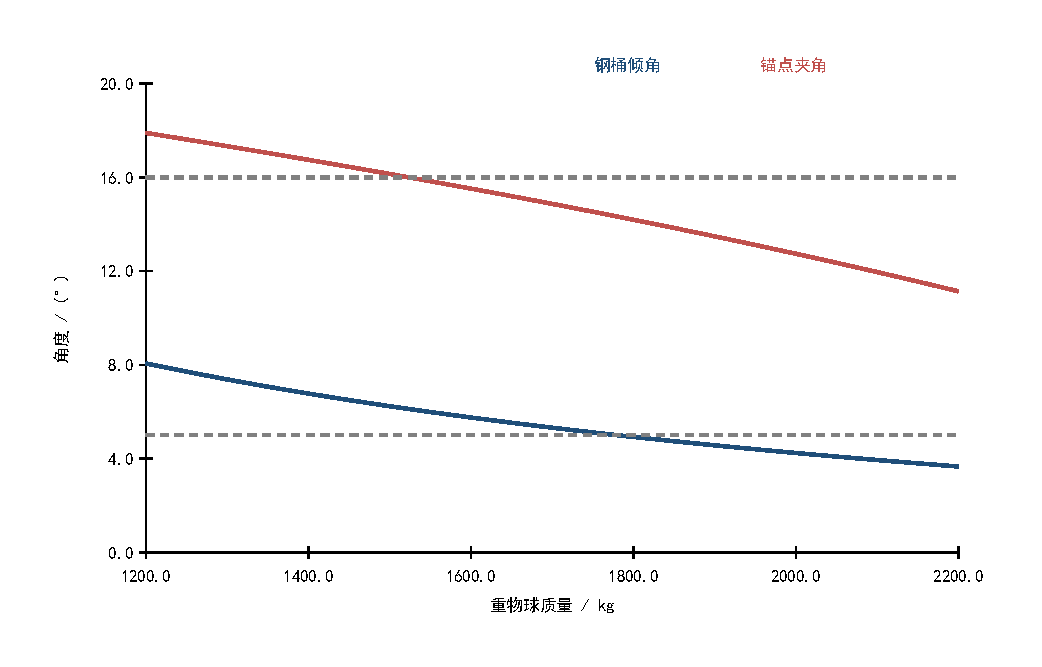
\includegraphics[width=0.78\textwidth]{../figures/question-2-ballast-sensitivity.pdf}
\caption{36 m/s风速下配重质量与角度约束的关系}
\label{fig:q2-mass}
\end{figure}
锚点夹角约束对应的临界质量为

\[
m_\alpha=1524.0332\ \mathrm{kg}.
\]
但此时钢桶倾角仍为 \(6.1176^\circ\)，不满足 \(5^\circ\) 要求。钢桶倾角约束对应的临界质量为

\[
m_\theta=1780.8803\ \mathrm{kg}.
\]
由于 \(m_\theta>m_\alpha\)，钢桶倾角约束是有效约束。因此

\[
\boxed{m_s\ge1780.8803\ \mathrm{kg}} \tag{24}
\]
为同时满足两个角度条件的质量范围，理论最优解为

\[
\boxed{m_s^*=1780.8803\ \mathrm{kg}}. \tag{25}
\]
\subsection{理论最优解的完整状态}
理论最优配重下，浮标吃水为0.9438 m，水平风荷载为1710.99 N，游动半径为18.4832 m；钢桶倾角和锚点夹角分别为$5.0000^\circ$和$14.3265^\circ$。
最优点的水深闭合关系为

\[
0.9438+12.0748+4.9814=18.0000\ \mathrm m.
\]
钢桶倾角恰好达到 \(5^\circ\)，锚点夹角比16°限制低 \(1.6735^\circ\)。因此理论最优解由钢桶倾角约束决定。

此时锚链参数为

\[
a=\frac{H}{q}=24.9161\ \mathrm m,
\qquad
b=\operatorname{arsinh}\frac{V_a}{H}=0.25269.
\]
锚链形状为

\[
y(x)=24.9161\left[
\cosh\left(\frac{x}{24.9161}+0.25269\right)
-\cosh(0.25269)
\right],
\]
其中

\[
0\le x\le18.0526.
\]
\subsection{1800 kg推荐方案}
理论最优解1780.8803 kg位于钢桶倾角约束边界，实际加工和配重配置通常取整，因此推荐采用

\[
\boxed{m_s=1800\ \mathrm{kg}}.
\]
1800 kg方案的浮标吃水为0.9496 m，水平风荷载为1701.71 N，游动半径为18.4768 m；钢桶倾角和锚点夹角分别为$4.9276^\circ$和$14.1945^\circ$。原方案、两个角度边界及推荐方案的吃水和锚链顶端张力变化见图\ref{fig:q2-state}。

\begin{figure}[H]\centering
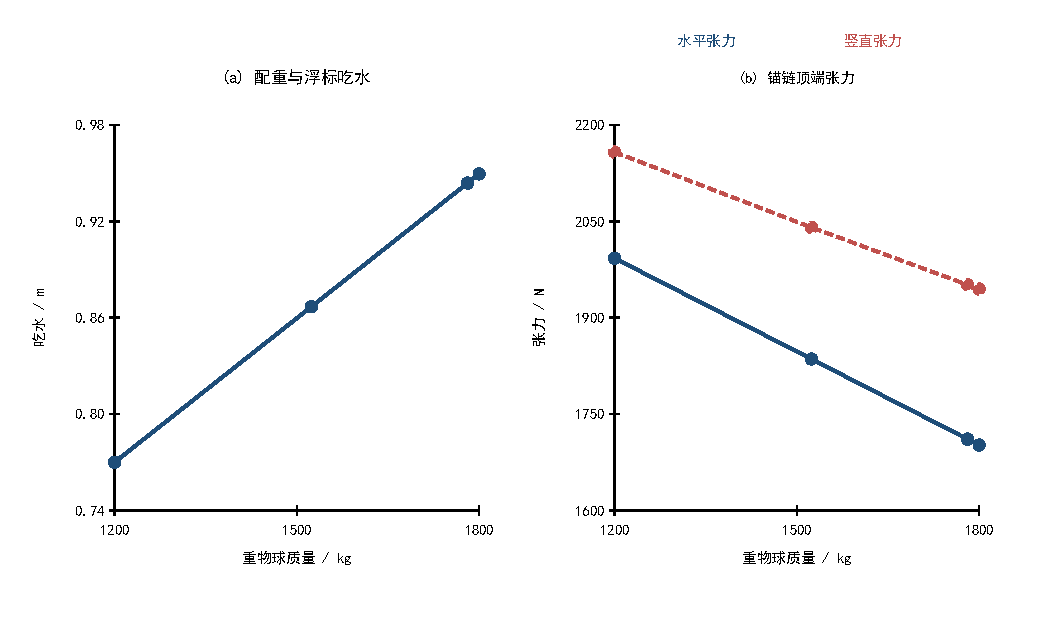
\includegraphics[width=0.95\textwidth]{../figures/question-2-state-comparison.pdf}
\caption{原方案、角度边界与推荐配重的吃水和张力比较}
\label{fig:q2-state}
\end{figure}
1800 kg方案满足

\[
4.9276^\circ<5^\circ,
\qquad
14.1945^\circ<16^\circ,
\]
并分别留有 \(0.0724^\circ\) 和 \(1.8055^\circ\) 的角度余量。

\subsection{结果检验与讨论}
首先，原1200 kg方案与优化方案均通过18 m水深闭合检验，程序的几何闭合误差小于 \(10^{-8}\) m。其次，随着配重质量增加，钢桶倾角、钢管倾角和锚点夹角均连续下降，符合配重提高竖直张力、减小构件偏转的物理规律。再次，最优解处钢桶约束恰好取等号，而锚点约束具有正余量，与“取两个单约束临界质量的较大者”的优化结构一致。

理论最优质量是确定性静力模型中的约束边界解，对载荷扰动和制造偏差缺少概率意义上的安全余量；二分搜索还依赖质量区间内响应连续且单调。因而本文同时报告理论临界质量和向上取整后的推荐质量，但推荐值仍不能替代动态与不确定性条件下的可靠性设计。

\subsection{配重敏感性与控制约束}
在1200--2200 kg扫描区间内，钢桶倾角和锚点夹角随配重连续下降，21个质量节点均为完全悬链状态，故可用二分法定位临界质量。钢桶角约束较晚满足，因而控制理论最优解；1800 kg相对临界值增加约19.12 kg，保留$0.0724^\circ$的钢桶角余量。

配重增加也使吃水由0.7700 m增至1.0696 m，因此不能只追求更小倾角。1800 kg是满足角度约束后的可实施取整值，而非覆盖动态载荷和材料误差的安全系数。

\subsection{本问结论}
36 m/s风速下，原1200 kg重物球方案的钢桶倾角为 \(8.0636^\circ\)，锚点夹角为 \(17.9006^\circ\)，均不满足题目要求。将重物球质量作为设计变量，以质量最小为目标，并联立完全悬链、刚性构件平衡、浮标平衡及18 m水深闭合关系，得到满足两个角度约束的质量范围为

\[
\boxed{m_s\ge1780.8803\ \mathrm{kg}}.
\]
理论最优质量为1780.8803 kg，此时钢桶倾角为 \(5.0000^\circ\)，锚点夹角为 \(14.3265^\circ\)。考虑实际配重取整，推荐采用1800 kg重物球；此时钢桶倾角为 \(4.9276^\circ\)，锚点夹角为 \(14.1945^\circ\)，两项约束均得到满足。
\aimark{4}


\section{问题三：风流耦合下的鲁棒设计}
\subsection{问题分析}
问题三要求在水深16—20 m、最大风速36 m/s和最大流速1.5 m/s条件下重新设计系泊系统，确定锚链型号、链长和重物球质量，并分析不同环境状态下浮标吃水、游动半径、钢桶与钢管倾角以及锚链形状。与前两问相比，本问同时包含离散设计变量、连续设计变量、环境不确定性和多个相互冲突的性能目标。

本问采用“空间风流载荷—刚性构件递推—分段悬链线—鲁棒筛选—Pareto折中”的总体路线。首先建立允许风向和流向不一致的水平向量模型；其次考虑钢管和钢桶姿态对迎流面积的反馈；然后在每个环境状态下自动判断锚链部分铺底或完全悬起；最后枚举完整链环组成的链长，搜索满足安全约束的配重，并利用Pareto前沿和理想点距离选择折中方案。

\subsection{设计变量与环境变量}
设计变量写为

\[
\boldsymbol x=(k,N,m_s),
\]
其中 \(k\) 为锚链型号，\(N\) 为链环数量，\(m_s\) 为重物球质量。若第 \(k\) 型锚链单环长度为 \(l_k\)，则锚链总长满足

\[
L_c=Nl_k,\qquad N\in\mathbb Z^+.
\]
环境状态写为

\[
\boldsymbol\xi=(d,v_w,v_c,\varphi),
\]
其中

\[
d\in[16,20],\quad
v_w\in[0,36],\quad
v_c\in[0,1.5],\quad
\varphi\in[0,\pi].
\]
\(\varphi\) 表示水流方向相对风向的水平夹角。计算中以风向作为全局 \(x\) 轴方向。

\subsection{模型假设}
系统在稳定风流作用下达到静态平衡；浮标依靠浮稳性保持竖直；钢管和钢桶是铰接刚性圆柱构件；重物球作为钢桶下端的集中载荷；锚链是均匀、不可伸长的柔索；海床水平且忽略摩擦。钢管和钢桶按外部圆柱体积计算浮力。由于题目没有提供重物球和锚链排水体积，也没有给出二者的迎流尺寸，模型忽略其浮力和水流力。

水流速度视为沿水深均匀分布，钢管和钢桶的水流合力作用于各自几何中心。因此水流力影响构件水平力平衡，但对构件中心不产生附加力矩。该假设适用于题目给出的近似水流力公式和缺少流速剖面数据的情形。

\subsection{风流空间载荷模型}
\subsubsection{浮标风荷载}
设浮标吃水为 \(h\)，露出水面的迎风面积为

\[
S_w=2(2-h).
\]
风荷载大小为

\[
F_w=0.625S_wv_w^2
=1.25(2-h)v_w^2. \tag{1}
\]
其向量为

\[
\boldsymbol F_w=(F_w,0).
\]
\subsubsection{浮标水流力}
浮标浸水部分在水流法平面的投影面积为

\[
S_{c,f}=2h,
\]
故浮标水流力为

\[
F_{c,f}=374(2h)v_c^2. \tag{2}
\]
令水流方向单位向量为

\[
\boldsymbol e_c=(\cos\varphi,\sin\varphi),
\]
则浮标下端连接处需要平衡的初始水平载荷向量为

\[
\boldsymbol H_0
=\boldsymbol F_w+F_{c,f}\boldsymbol e_c. \tag{3}
\]
\subsubsection{倾斜圆柱的迎流面积}
设第 \(i\) 个刚性构件的倾角为 \(\theta_i\)，水平偏转单位向量为 \(\boldsymbol e_i\)。其空间轴向单位向量可写为

\[
\boldsymbol u_i=
(\sin\theta_i e_{i,x},
\sin\theta_i e_{i,y},
\cos\theta_i).
\]
构件轴线与水平水流方向的夹角决定其法平面投影。忽略较小的端面投影后，有

\[
S_{c,i}=d_iL_i
\sqrt{1-(\boldsymbol u_i\cdot\boldsymbol e_c)^2}. \tag{4}
\]
相应水流力为

\[
\boldsymbol F_{c,i}
=374S_{c,i}v_c^2\boldsymbol e_c. \tag{5}
\]
式（4）—式（5）体现了构件姿态与水流力之间的非线性反馈。

\subsection{钢管和钢桶的空间受力递推}
设某构件上端和下端承担的水平载荷向量分别为 \(\boldsymbol H_u\) 和 \(\boldsymbol H_l\)。从浮标向锚链方向递推时，该构件自身水流力需要由下方系泊系统继续承担，因此

\[
\boldsymbol H_l
=\boldsymbol H_u+\boldsymbol F_{c,i}. \tag{6}
\]
设其上下端竖直张力为 \(V_u,V_l\)，有效重量为 \(W_i\)，则

\[
V_u=V_l+W_i. \tag{7}
\]
对构件中心列空间力矩平衡，可以得到构件偏转方向与平均水平载荷方向一致：

\[
\boldsymbol e_i=
\frac{\boldsymbol H_u+\boldsymbol H_l}
{\|\boldsymbol H_u+\boldsymbol H_l\|}, \tag{8}
\]
倾角满足

\[
\tan\theta_i=
\frac{\|\boldsymbol H_u+\boldsymbol H_l\|}
{V_u+V_l}. \tag{9}
\]
由于式（4）的投影面积依赖 \(\theta_i\) 和 \(\boldsymbol e_i\)，程序对式（4）—式（9）进行不动点迭代，直至相邻两次构件倾角变化小于 \(10^{-12}\) rad。

重物球仍作为钢桶下端独立集中载荷。设锚链顶端竖直张力为 \(V_t\)，则钢桶下端竖直载荷为

\[
V_{b,l}=V_t+m_sg.
\]
四节钢管的竖直张力从钢桶向浮标逐节增加，浮标吃水为

\[
h=\frac{1000g+V_t+m_sg+W_b+4W_p}{\rho g\pi}. \tag{10}
\]
\subsection{锚链状态与空间位置}
锚链本身没有水平分布载荷，其水平张力方向由钢桶下端水平载荷向量决定。令

\[
H_c=\|\boldsymbol H_c\|,
\qquad
\boldsymbol e_H=\frac{\boldsymbol H_c}{H_c}.
\]
在由 \(\boldsymbol e_H\) 和竖直方向组成的局部平面内，锚链仍满足悬链线方程。程序首先尝试部分铺底模型：令锚点竖直张力为零，以悬起链长为未知量求水深闭合。如果所需悬起长度不超过总链长，则保留铺底状态；否则切换为完全悬链模型，并以锚点竖直张力为未知量求解。

完全悬链状态下，锚点夹角为

\[
\alpha_a=\arctan\frac{V_a}{H_c}. \tag{11}
\]
锚链水平位移沿 \(\boldsymbol e_H\) 方向，再与五个刚性构件的水平投影向量相加，得到浮标相对锚点的水平位移向量。其模长定义为游动半径：

\[
R=\|\boldsymbol r_f-\boldsymbol r_a\|. \tag{12}
\]
\subsection{鲁棒约束与多目标函数}
对所有设计工况，要求

\[
\theta_b\le5^\circ,
\qquad
\alpha_a\le16^\circ. \tag{13}
\]
问题要求吃水、游动区域和钢桶倾角尽可能小，因此定义最坏工况目标

\[
J_1(\boldsymbol x)=\max_{\boldsymbol\xi}h,
\]
\[
J_2(\boldsymbol x)=\max_{\boldsymbol\xi}R,
\]
\[
J_3(\boldsymbol x)=\max_{\boldsymbol\xi}\theta_b. \tag{14}
\]
不直接设置主观权重，而是先进行Pareto支配筛选。若设计A在三个目标上均不差于设计B，且至少一个目标严格更优，则删除B。对于剩余Pareto方案，将三个目标分别归一化到 \([0,1]\)，计算其到理想点 \((0,0,0)\) 的欧氏距离：

\[
D(\boldsymbol x)=
\sqrt{\hat J_1^2+\hat J_2^2+\hat J_3^2}. \tag{15}
\]
选择 \(D\) 最小的方案作为折中设计。

\subsection{搜索与验证设置}
五种锚链型号全部参与搜索，链长范围扩展为18—32 m，并严格按完整链环数量取值。为控制混合搜索规模，在约0.5 m的链长带宽上进行初筛。对每组链型和链长，先在16 m和20 m水深、36 m/s风速、1.5 m/s流速、风流同向条件下搜索满足式（13）的最小配重，再增加0、200和400 kg三个配重余量档位形成多目标候选集。

初筛共得到204个可行候选和97个Pareto方案。对折中方案进一步遍历

\[
d\in\{16,18,20\},
\quad v_w\in\{12,24,36\},
\]
\[
v_c\in\{0,0.5,1.0,1.5\},
\quad\varphi\in\{0^\circ,45^\circ,90^\circ,135^\circ,180^\circ\},
\]
共180个验证工况。结果显示各指标最坏值均出现在36 m/s、1.5 m/s和风流同向条件；风流夹角增大后水平合力和构件倾角下降。这支持用同向极端风流作为设计筛选工况。

\subsection{优化结果与推荐设计}
理想点距离最小的Pareto方案为：

\[
\boxed{
k=\mathrm{IV},\quad N=147,
\quad L_c=147\times0.150=22.05\ \mathrm m
}
\]
其Pareto计算配重为4006.91 kg。考虑配重实施和安全余量，将质量向上取整到50 kg档位，得到推荐设计

\[
\boxed{
\text{IV型锚链22.05 m，重物球4050 kg}
}. \tag{16}
\]
推荐方案在180个验证工况中的最坏指标为：

\begin{table}[H]\centering\small
\caption{推荐方案的鲁棒验证结果}
\label{tab:q3-1}
\resizebox{\textwidth}{!}{%
\begin{tabular}{cccccc}
\toprule
指标 & 最坏值 & 对应水深/m & 风速/(m/s) & 流速/(m/s) & 风流夹角 \\
\midrule
浮标吃水/m & 1.7519 & 20 & 36 & 1.5 & 0° \\
游动半径/m & 19.6195 & 16 & 36 & 1.5 & 0° \\
钢桶倾角/(°) & 4.7382 & 16 & 36 & 1.5 & 0° \\
锚点夹角/(°) & 14.8547 & 20 & 36 & 1.5 & 0° \\
\bottomrule
\end{tabular}
}
\end{table}
最坏钢桶倾角和锚点夹角分别保留

\[
5^\circ-4.7382^\circ=0.2618^\circ,
\]
\[
16^\circ-14.8547^\circ=1.1453^\circ
\]
的余量。

\subsection{不同水深下的极端同向风流状态}
在36 m/s风速、1.5 m/s流速且风流同向时，推荐方案的水深响应见图\ref{fig:q3-depth}。

\begin{figure}[H]\centering
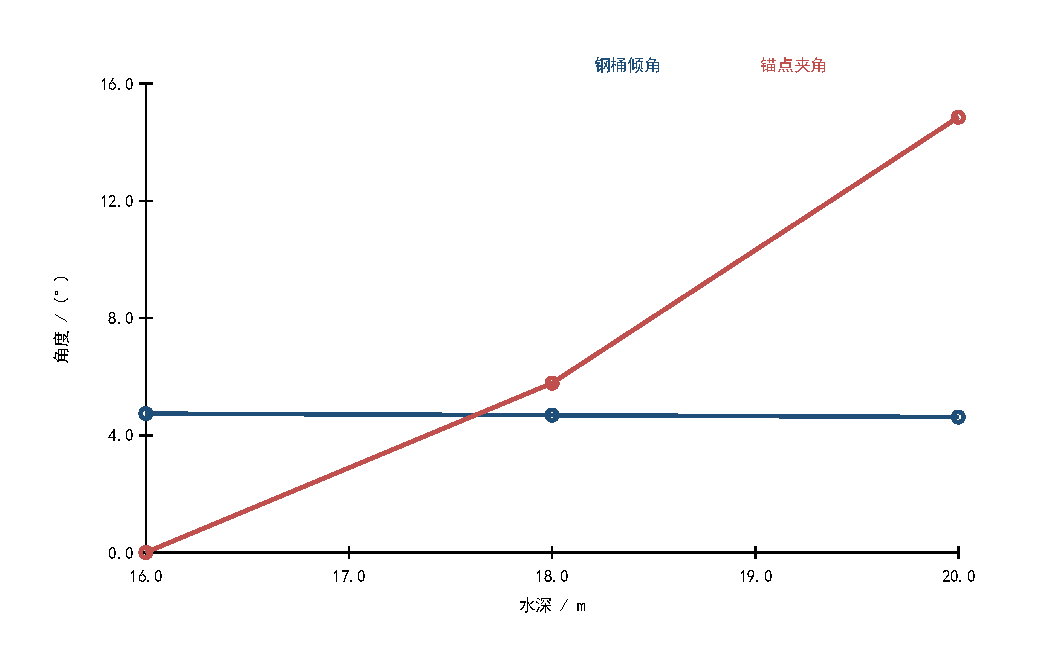
\includegraphics[width=0.78\textwidth]{../figures/question-3-depth-angles.pdf}
\caption{推荐方案在最大同向风流下的水深--角度响应}
\label{fig:q3-depth}
\end{figure}
浅水时存在铺底链段，锚点切线水平，所以锚点夹角为零；同时较长的海床铺展使游动半径达到最大。深水时整条锚链悬起，锚点竖直张力明显增加，因而锚点夹角在20 m水深达到最大。钢桶倾角则在浅水16 m达到最大。这说明问题三不存在一个对所有指标都统一最不利的水深端点。

\subsection{风速变化的影响}
为单独考察风速作用，固定水深18 m、水流速度1.5 m/s，并令风流方向相同。角度响应见图\ref{fig:q3-environment}(a)。
风速从12 m/s增至36 m/s后，钢桶倾角由 \(4.1969^\circ\) 增至 \(4.6834^\circ\)，游动半径由18.4785 m增至18.6692 m，锚点夹角由 \(2.9265^\circ\) 增至 \(5.7781^\circ\)。风荷载与风速平方成正比，因此水平张力随风速增加；但是浮标吃水仅增加0.0066 m，说明风速主要改变水平受力，而对系统竖直载荷的影响相对较弱。

\subsection{水流速度变化的影响}
固定水深18 m、风速36 m/s和风流同向，改变水流速度，角度响应见图\ref{fig:q3-environment}(b)。
流速由0增至1.5 m/s时，钢桶倾角由 \(0.7192^\circ\) 增至 \(4.6834^\circ\)，游动半径增加3.9679 m，锚链由部分铺底转换为完全悬起。水流影响显著的原因有两点：水流力与流速平方成正比；水流同时作用于浮标浸水部分、四节钢管和钢桶，其水平载荷沿构件向锚链逐节累积。尤其当流速由1.0 m/s增至1.5 m/s时，水流力增为原来的2.25倍，并触发锚链状态转换，使锚点出现非零竖直张力。

\subsection{风流夹角的影响}
固定水深18 m、风速36 m/s和流速1.5 m/s，改变风流夹角，角度响应见图\ref{fig:q3-environment}(c)。

\begin{figure}[H]\centering
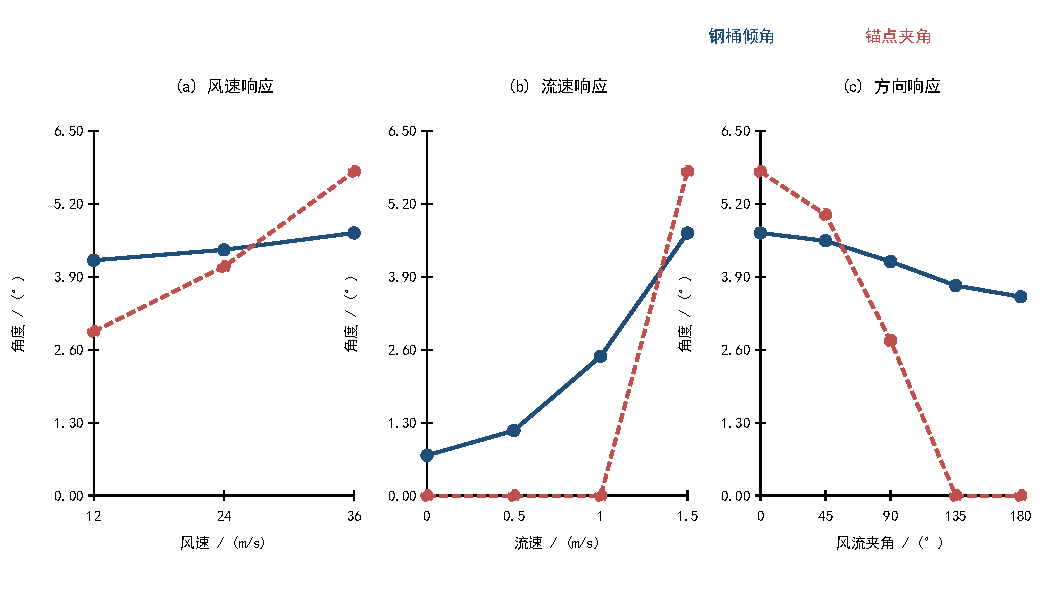
\includegraphics[width=0.98\textwidth]{../figures/question-3-environmental-response.pdf}
\caption{推荐方案对风速、流速和风流夹角的角度响应}
\label{fig:q3-environment}
\end{figure}
随着风流夹角由 \(0^\circ\) 增至 \(180^\circ\)，钢桶倾角和游动半径总体下降。同向风流下两类水平载荷叠加，系统水平合力最大；反向时风力和水流力部分抵消。当夹角达到 \(135^\circ\) 后，锚链重新出现铺底段，锚点切线角降为零。因此最大风速、最大流速且风流同向是方向组合中的最不利状态。

\subsection{钢管倾角和钢桶倾角的分布规律}
在相同工况下，第1节至第4节钢管倾角依次增加，钢桶倾角最大。例如在16 m水深的极端同向风流下，四节钢管倾角依次为

\[
4.3446^\circ,\quad4.4062^\circ,
\quad4.4681^\circ,\quad4.5301^\circ,
\]
钢桶倾角为

\[
4.7382^\circ.
\]
越靠近浮标的钢管承担越大的竖直张力，因此在相近水平载荷下更加接近竖直。钢桶的直径为0.30 m，是钢管直径0.05 m的6倍，其迎流面积和水流力明显更大；虽然重物球提高了钢桶两端竖直张力，钢桶倾角仍略高于各节钢管。因此钢桶倾角可以作为水声通讯设备工作状态的控制指标。

\subsection{锚链形状与状态转换}
锚链形状随水深和水平环境载荷变化，并非始终属于同一种悬链状态。部分铺底时，锚链由海床水平段和悬链线段组成。若铺底长度为 \(L_g\)，则

\[
y=0,\qquad 0\le x\le L_g,
\]
悬起部分可写为

\[
y=a\left[
\cosh\left(\frac{x-L_g}{a}\right)-1
\right], \tag{16}
\]
其中 \(a=H_c/q\)。完全悬起时，锚点竖直张力 \(V_a>0\)，锚链形状为

\[
y=a\left[
\cosh\left(\frac{x}{a}+b\right)-\cosh b
\right], \tag{17}
\]
其中

\[
b=\operatorname{arsinh}\frac{V_a}{H_c}.
\]
在最大同向风流下，16 m水深时有0.7710 m锚链铺在海床上，锚点切线水平；18 m和20 m水深时整条锚链悬起。20 m水深需要更大的锚链竖直跨度，因此链形更加陡峭，锚点夹角达到 \(14.8547^\circ\)。从流速变化也可以观察到相同转换：水深18 m时，流速不超过1.0 m/s仍有铺底链段，流速达到1.5 m/s后整链悬起。

图\ref{fig:q3-depth}采用统一坐标尺度比较最大同向风流下的水深响应，使铺底状态、锚点夹角与钢桶倾角的控制水深能够直接对应。

\subsection{游动区域与最坏工况汇总}
浮标保持竖直时，其轴线水平位置与底部连接点一致。风流方向变化使系统绕锚点改变水平偏转方向，因此用水平偏移模长 \(R\) 表示游动半径，游动圆面积为

\[
A_R=\pi R^2. \tag{18}
\]
推荐方案的最大游动半径为19.6195 m，因此最大游动区域面积为

\[
A_{R,\max}=\pi(19.6195)^2
\approx1209.5\ \mathrm{m^2}.
\]
\begin{table}[H]\centering\small
\caption{推荐方案的最坏工况及约束校核}
\label{tab:q3-6}
\resizebox{\textwidth}{!}{%
\begin{tabular}{cccc}
\toprule
指标 & 最坏值 & 对应工况 & 限制或目标 \\
\midrule
钢桶倾角 & \(4.7382^\circ\) & 16 m、36 m/s、1.5 m/s、同向 & 不超过 \(5^\circ\) \\
锚点夹角 & \(14.8547^\circ\) & 20 m、36 m/s、1.5 m/s、同向 & 不超过 \(16^\circ\) \\
浮标吃水 & 1.7519 m & 20 m、36 m/s、1.5 m/s、同向 & 尽可能小且小于2 m \\
游动半径 & 19.6195 m & 16 m、36 m/s、1.5 m/s、同向 & 尽可能小 \\
游动圆面积 & 约1209.5 m² & 同最大游动半径工况 & 尽可能小 \\
\bottomrule
\end{tabular}
}
\end{table}
由表\ref{tab:q3-6}可知，不同指标对应不同的最不利水深。浅水增加锚链沿海床的水平展开长度，主要控制游动区域和钢桶倾角；深水增加锚链的竖直跨度和锚点竖直张力，主要控制吃水和锚点夹角。因此不能只选择单一水深作为所有指标的最坏工况。

\subsection{模型检验和局限}
所有输出工况均通过相应水深的几何闭合检验，程序闭合误差控制在 \(10^{-8}\) m量级；锚链铺底和全悬状态由求解结果自动判别。将搜索范围由20—28 m扩大到18—32 m后，折中方案仍位于区间内部的22.05 m，说明推荐链长不是由原搜索边界强制产生。

模型采用准定常阻力和均匀流速近似，未描述构件尾流遮蔽、涡激振动及姿态变化引起的非定常流固耦合；锚链的理想柔索表达也忽略链环弹性与海床接触滞回。风流连续区间仅由端点筛选和180个代表工况验证，不能构成连续四维环境域的严格全局证明。后续可采用时域刚柔耦合模型、自适应环境采样和弹性链环接触模型复核推荐方案。

\subsection{候选设计分布与折中方案证据}
初筛得到204个可行候选，Pareto筛选后保留97个非支配设计。在吃水、游动半径和钢桶倾角归一化后，IV型147环、22.05 m方案的理想点距离最小；加入200 kg配重余量并取整后推荐4050 kg。该结果是当前多目标口径下的代表性折中，并非脱离偏好权重的唯一最优。

\subsection{验证工况覆盖与状态占比}
180个验证工况覆盖3个水深、3个风速、4个流速和5个风流夹角，其中152个为部分铺底、28个为完全悬起。全体工况的吃水、游动半径、钢桶倾角和锚点夹角范围分别为1.6454--1.7519 m、9.8107--19.6195 m、$0.0803^\circ$--$4.7382^\circ$和$0^\circ$--$14.8547^\circ$；各最坏值均可追溯到实际工况记录。

\subsection{本问结论}
通过空间风流水平载荷、姿态相关迎流面积、刚性构件递推、锚链状态切换和Pareto多目标搜索，得到问题三推荐设计为

\[
\boxed{
\text{IV型锚链，长度22.05 m，重物球质量4050 kg}
}.
\]
在所验证的水深16—20 m、风速不超过36 m/s、流速不超过1.5 m/s及不同风流夹角组合下，最坏钢桶倾角为 \(4.7382^\circ\)，最坏锚点夹角为 \(14.8547^\circ\)，均满足题目限制。最大吃水为1.7519 m，最大游动半径为19.6195 m。浅水主要控制游动半径和钢桶倾角，深水主要控制吃水和锚点夹角。
\aimark{5}


\section{统一求解与适用边界}

\subsection{状态判别与数值闭合}

三问共用浮标、刚性构件和锚链静力模型。给定环境与设计变量后，程序由下向上递推竖直张力和构件倾角，再用水深条件闭合吃水、锚链高度与各段竖直投影。锚链先按部分铺底分支求解；若所需悬起长度超过总链长，则切换到完全悬起分支并引入锚点竖直张力。该处理避免预先固定锚链状态造成不相容解。

问题二在静力求解器外对配重质量作区间搜索，分别求钢桶倾角和锚点夹角的临界质量并取较大者；问题三枚举链型、链环数和配重档位，再对候选方案作多工况复核。每个结果均检查水深闭合、受力平衡、吃水范围和锚链状态，问题一另以210链环离散模型校核连续悬链线近似。

\subsection{模型边界}

统一模型采用准静态、不可伸长柔索和准定常阻力近似，不能反映结构惯性、链环弹性、海床接触滞回及风流脉动造成的瞬态响应。状态切换由解析边界判定，在临界离床区域可能放大数值不光滑性；代表工况枚举也只验证离散环境集合。因而本文结论用于稳态方案比较，不能替代时域动力学、接触力学和连续不确定环境下的鲁棒性分析。


\section{模型评价与改进}
本文模型把浮标吃水、风载面积、刚性构件姿态和锚链边界状态置于同一闭合框架中，能够解释风速增加、配重变化和水深变化如何沿系统传递。问题三使用水平向量而非简单标量叠加，可分析非同向风流；链长严格由完整链环组成，最终设计具有可实施的离散结构。连续悬链线与离散链环结果的一致性，为大量工况下采用解析链形提供了计算依据。

模型的首要局限是准静态平衡无法描述阵风、波浪激励下的瞬态峰值、惯性效应和疲劳累积，因而推荐方案只反映稳态载荷水平。其次，理想不可伸长柔索忽略链环轴向弹性、弯曲刚度、海床接触摩擦与局部冲击，使铺底和全悬之间被处理为理想状态切换。再次，均匀流速和准定常阻力模型未刻画尾流遮蔽、构件间流体耦合及姿态变化引起的时变阻力。问题三的离散工况搜索也不能严格证明连续环境域内的全局鲁棒性，Pareto理想点还对归一化范围敏感。后续可建立刚柔耦合时域模型，引入弹性离散链及接触摩擦，并在连续环境域上采用自适应采样和鲁棒优化复核方案。
\aimark{6}

\begin{thebibliography}{9}
\bibitem{catenary} Irvine H M. Cable Structures[M]. Cambridge: MIT Press, 1981.
\bibitem{mechanics} 哈尔滨工业大学理论力学教研室. 理论力学[M]. 北京: 高等教育出版社, 2016.
\bibitem{ai} OpenAI. Codex，模型与程序辅助工具，使用日期：2026-08-01.
\end{thebibliography}

\CumcmMainMatterEnd
\appendix
\ctexset{section={name={附录,、},number=\Alph{section}}}
\section{支撑材料与代码说明}

\begingroup
\renewcommand{\texttt}[1]{{\ttfamily\seqsplit{#1}}}
\scriptsize
\setlength{\tabcolsep}{2pt}
\begin{longtable}{L{0.12\textwidth}L{0.18\textwidth}L{0.28\textwidth}L{0.32\textwidth}}
\caption{各问题关键小点与可运行代码文件清单}\label{tab:appendix-code}\\
\toprule 对应问题 & 关键小点 & 文件名 & 用途\\ \midrule
\endfirsthead
\toprule 对应问题 & 关键小点 & 文件名 & 用途\\ \midrule
\endhead
问题一 & 静力平衡 & \texttt{solve\_question1.py} & 求两种风速下的系统状态\\
问题一 & 离散校核 & \texttt{validate\_discrete\_chain.py} & 210链环离散模型复算\\
问题二 & 原方案判断 & \texttt{solve\_question2.py} & 复算36 m/s原配重方案\\
问题二 & 临界质量搜索 & \texttt{solve\_question2.py} & 搜索两个角度约束边界\\
问题二 & 敏感性分析 & \texttt{solve\_question2.py} & 扫描配重与约束指标\\
问题三 & 风流耦合求解 & \texttt{solve\_question3.py} & 计算空间载荷和锚链状态\\
问题三 & 候选设计枚举 & \texttt{solve\_question3.py} & 枚举链型、链环数和配重\\
问题三 & Pareto筛选 & \texttt{solve\_question3.py} & 选取非支配折中方案\\
问题三 & 多工况复核 & \texttt{solve\_question3.py} & 复核推荐方案180个工况\\
共用 & 论文图形生成 & \texttt{generate\_figures.py} & 从结果数据生成五幅论文图\\
\bottomrule
\end{longtable}

\begin{longtable}{L{0.12\textwidth}L{0.34\textwidth}L{0.42\textwidth}}
\caption{关键数据、结果与图形文件清单}\label{tab:appendix-data}\\
\toprule 对应问题 & 文件名 & 用途\\ \midrule
\endfirsthead
\toprule 对应问题 & 文件名 & 用途\\ \midrule
\endhead
问题一 & \texttt{question-1-summary.csv} & 两种风速下的系统平衡汇总\\
问题一 & \texttt{chain-profiles.csv} & 两种风速下的锚链离散坐标\\
问题一 & \texttt{continuous-discrete-validation.csv} & 连续悬链线与210链环模型误差\\
问题二 & \texttt{question-2-summary.csv} & 原方案、两个临界质量和推荐方案结果\\
问题二 & \texttt{ballast-mass-sensitivity.csv} & 1200--2200 kg配重扫描结果\\
问题三 & \texttt{design-candidates.csv} & 204个可行候选设计及其最坏响应\\
问题三 & \texttt{pareto-designs.csv} & 97个Pareto非支配设计\\
问题三 & \texttt{selected-design-summary.csv} & 推荐设计与最坏指标汇总\\
问题三 & \texttt{selected-design-scenarios.csv} & 推荐方案180个验证工况\\
问题一 & \texttt{question-1-chain-profiles.pdf} & 两种风速下的锚链形状图\\
问题二 & \texttt{question-2-ballast-sensitivity.pdf} & 配重质量与角度约束关系图\\
问题二 & \texttt{question-2-state-comparison.pdf} & 原方案、临界方案与推荐方案的状态对比图\\
问题三 & \texttt{question-3-depth-angles.pdf} & 最大同向风流下水深--角度响应图\\
问题三 & \texttt{question-3-environmental-response.pdf} & 风速、流速与风流夹角响应图\\
全文 & AI 工具使用详情.pdf & 记录AI辅助范围、关键交互、采纳内容与人工核验\\
\bottomrule
\end{longtable}
\endgroup
\end{document}
